\documentclass[a4paper,pdf]{article} % gebruik acm style voor je scriptie: [format=acmsmall, screen=true, review=false]{acmart} 


%\documentclass[sigconf]{acmart} 
%\documentclass[sigconf,format=acmsmall, screen=true, review=false]{acmart} 
\usepackage{amsmath}
\usepackage{amsfonts}
\usepackage{amssymb}
\usepackage{hyperref}
\usepackage{pdfpages} % http://mirror.unl.edu/ctan/macros/latex/contrib/pdfpages/pdfpages.pdf
\usepackage{booktabs} 


\usepackage[utf8]{inputenc}
\usepackage{graphicx}
\graphicspath{ {./images/} }
\usepackage[colorinlistoftodos]{todonotes} % handig voor commentaar: gebruik \todo{}, zie ftp://ftp.fu-berlin.de/tex/CTAN/macros/latex/contrib/todonotes/todonotes.pdf
\usepackage{listings}
\usepackage{multirow}
\usepackage{tcolorbox}
\usepackage{float}
\usepackage{caption}
\usepackage{subcaption}

% Add numbering for paragraphs
\usepackage{titlesec}
\setcounter{secnumdepth}{4}
\titleformat{\paragraph}
{\normalfont\normalsize\bfseries}{\theparagraph}{1em}{}
\titlespacing*{\paragraph}
{0pt}{3.25ex plus 1ex minus .2ex}{1.5ex plus .2ex}

% when writing in Dutch
%\usepackage[dutch]{babel}
%\selectlanguage{dutch}


% linenumbering  See https://texblog.org/2012/02/08/adding-line-numbers-to-documents/
% \usepackage{lineno}
% \linenumbers

\newcommand{\shorttitle}{} % Put your short title here
\begin{document}

\begin{center}

\vspace{2.5cm}

% [CHANGE] The title of your thesis. If your thesis has a subtitle, then this
% should appear right below the main title, in a smaller font.
\begin{Huge}
Fake news: an algorithmic perspective on fact-checking
\end{Huge}

\vspace{1.5cm}

% [CHANGE] Your full name. In case of multiple names, you can include their
% initials as well, e.g. "Jan G.J. van der Wegge".
Martijn B.J. Schouten\\
% [CHANGE] Your student ID, as this has been assigned to you by the UvA
% administration.
11295562

\vspace{1.5cm}

% [DO NOT CHANGE]
Bachelor thesis\\
% Whether your Bachelor thesis is 6 ECTS (regular) or 9 ECTS (Honours
% programme).
Credits: 12 EC

\vspace{0.5cm}

% [DO NOT CHANGE] The name of the educational programme.
Bachelor's degree Information Science

\vspace{0.25cm}

% [DO NOT CHANGE] The addess of the educational programme.
University of Amsterdam\\
Faculty of Science\\
Science Park 904\\
1098 XH Amsterdam

\vspace{4cm}

\emph{Supervisor}\\
% The name of your supervisor. Include the titles of your supervisor,
% as well as the initials for *all* of his/her first names.
Dr. M. J. Marx

\vspace{0.25cm}

% The address of the institute at which your supervisor is working.
% Be sure to include (1) institute (is appropriate), (2) faculty (if
% appropriate), (3) organisation name, (4) organisation address (2 lines).
ILPS, IvI\\
Faculty of Science\\
University of Amsterdam\\
Science Park 904\\
1098 XH Amsterdam

\vspace{1.5cm}

% The date at which you will finalize and submit your thesis.
2019-06

\end{center}


\pagebreak

%\todototoc
%\listoftodos

\pagebreak

\begin{abstract}
% [CHANGE] 
\todo{Add an abstract}
\end{abstract}

\pagebreak

\tableofcontents

\pagebreak

% Here you input all your sections in seperate files

In the pre-Internet era, the ability to broadcast information on a large scale was in the hands of large publishing organizations. 
Nowadays, everyone can share news and information via social media with the possibility of reaching a large, global audience \cite{howell2013}. 
This introduces risks on validity and authenticity of news, as social media and digital platforms can speed up the spread of falsehoods without requiring much effort from the author \cite{europeancommission2018}. 

As a matter of fact, 63\% of adults in the United States prefer to read their news on the Internet. 
Young adults take the lead: 76\% of adults between the ages 18 and 49 get their primary news consumption via the web, compared to just 43\% for adults of 50 years and older \cite{mitchell2018}.
As time passes by, social media is slowly becoming the primary source of news for more and more people. 

The main danger of this development is that human perception is often skewed with regards to objectivity of facts. 
Psychological human traits such as naïve realism let consumers of news belief that their perception is right, while other's perceptions are uninformed. 
Furthermore, confirmation bias results in consumers preferring information that confirms beliefs they already have \cite{shu2017}. 
This makes consumers vulnerable for the spread of misinformation or fake news. 

According to the European Commission, \textit{"disinformation - or fake news - consists of verifiably false or misleading information that is created, presented and disseminated for economic gain or to intentionally deceive the public, and may cause public harm"} \cite{europeancommission2018}. 
The answer to the problem of fake news as of recently has been to manually fact-check statements on validity, but, as Shu et al. underlines, one of the downsides to this approach is that fake news typically relates to newly emerging, time-critical events. 
This means the real news may not be fully verified by proper knowledge bases due to a lack of contradicting claims \cite{shu2017}. 
An automated approach would both help in solving the problem of human subjectivity and the speed at which false information is spread in the current news consumption landscape.
Furthermore, such an approach can help human fact-checking by targetting statements that are most likely to be false.

Natural language processing has been in rapid development over the past years. 
With the releases of OpenAI's GPT-2 model in February of this year and Google's BERT in the autumn of 2018, state-of-the-art pre-trained textual embedding techniques have shown promising results on various classification tasks \cite{radford2019}\cite{devlin2018}. 
Although fake news classification has been attempted before \cite{wang2018}\cite{khurana2017}, performance on these classifiers has been rather low. 
However, these new pre-trained textual embeddings have not yet been used in the fight against disinformation. 

This paper is focussed on the following research question: \textit{what is the performance of combinations of pre-trained embedding techniques with machine learning algorithms when classifying fake news?}
This main question will be answered through the results of the following subquestions:

\begin{description}
\item[RQ1] Which way of pooling vectors to a fixed length works best for classifying fake news?
\item[RQ2] At what maximum sequence length do neural networks hold the highest accuracy when classifying fake news?
\item[RQ3] How well do neural network classification architectures classify fake news compared to non-neural classification algorithms?
\end{description}

The structure of this paper will be as follows: first, related work regarding fake news detection, pre-trained word embeddings and preparing text for classification will be discussed.
Then, the methodology will be laid out, including throughout explanation of our pre-trained embedding methods. 
To conclude, these embedding techniques will be applied to the Liar dataset and classification results will be shared.
\section{Related Work}

\subsection{RQ1}
Fake news as a term only caught public attention starting from the end of 2016, during the Presidential Elections of the United States \cite{googletrends2019}.   

\subsection{RQ2}
In the last couple of years, using transfer learning for natural language processing has given promisable results. The following sentence embeddings will be used to detect fake news:

\begin{itemize}
    \item Bag of Words as a baseline for performance of non-pretrained embeddings;
    \item Facebook's InferSent \cite{conneau2017};
    \item ELMo from the Allen Institute for Artificial Intelligence \cite{peters2018};
    \item OpenAI's GPT-2 \cite{radford2019};
    \item Transformer-XL \cite{dai2019};
    \item Microsoft's MT-DNN  \cite{liu2019};
    \item and Google's BERT \cite{devlin2018}.
\end{itemize}

\subsection{RQ3}
Aligned with the original research on this dataset by Wang \cite{wang2018}, the following machine learning algorithms will be used to test the applicability of the abovementioned embedding techniques: 
\begin{itemize}
    \item SVMs;
    \item Logistic regression;
    \item Bi-LSTMs;
    \item CNNs.
\end{itemize}
\section{Methodology}

\subsection{Description of the data}
% Data verzameling en beschrijving van de data
% Hoe is de data verzameld, en hoe heb jij die data verkregen?
% Wat staat er in de data? Niet alleen maar een technisch verhaal, maar ook inhoudelijk. DE lezer moet een goed idee krijgen over de technische inhoud en wat het betekent.
For classifying fake news, Wang's Liar dataset will be used \cite{wang2018}. 
The Liar dataset contains 12.791 short statements from Politifact.com, which are labeled manually by a Politifact.com editor on truthfulness. 
The statements are an average of 18 tokens long, and the topics vary from different political subjects, as can be seen in figure 1\todo{Check whether this number is still correct}.
Truthfulness is evaluated by assigning one of 6 labels, ranging from \textit{pants-on-fire} to \textit{true}. 
The distribution of statements across labels can be seen in figure X\todo{Create a figure comparing distributions of labels before and after preprocessing and insert the right figure number}. 

\begin{figure}[h]
    \centering
    
\includegraphics[scale=0.25]{subjectwordcloud}
    \caption{An overview of all statement topics in the Liar dataset.}
\end{figure}

For each statement, the dataset contains an id, a label, a subject, a speaker, the function title of the speaker, the affiliated state and political affiliation, the context of the statement and a vector with a truthfulness history.
Wang introduced this truthfulness history to boost the prediction scores, as speakers with a track record of lying are expected to have a lower chance of speaking the truth when classifying new statements.
However, for our application we are only interested in the statement itself and its corresponding label. 
Due to cheapness and spreadability, a large amount of fake news is spread over social media \cite{shu2017}. 
This means author information and metadata will not readily be available in real world circumstances.

The original dataset has been split beforehand into a test, train and validation set. 
The train set contains 80\% of the total amount of statements, while the test and validation set both contain approximately 10\% of the statements. 

\begin{figure}[h]
    \centering
    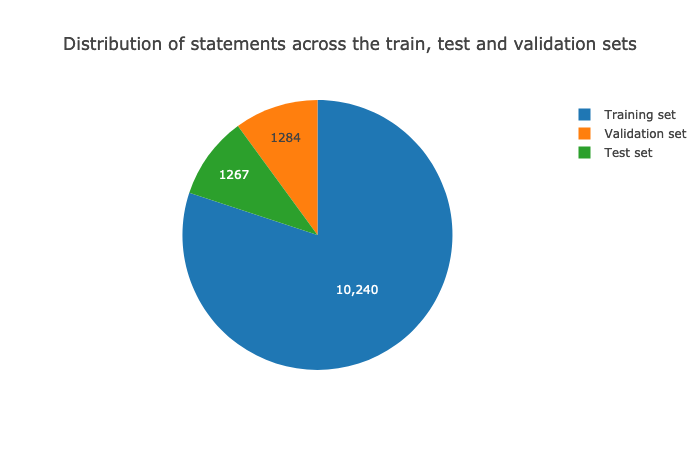
\includegraphics[scale=0.5]{folddistribution}
    \caption{Distribution of the total dataset.}
\end{figure}


\subsection{Data}
% Plotjes

\subsection{Methods}
% Hoe je je vraag gaat beantwoorden.
% Dit is de langste sectie van je scriptie. 
% Als iets erg technisch wordt kan je een deel naar de Appendix verplaatsen. 
% Probeer er een lopend verhaal van te maken.
% Het is heel handig dit ook weer op te delen nav je deelvragen:

\subsubsection{RQ1}

\subsubsection{RQ2}

\subsubsection{RQ3}

\section{Evaluation}
% Met een subsectie voor elke deelvraag.
% In hoeverre is je vraag beantwoord?
% Een mooie graphic/visualisatie is hier heel gewenst.
% Hou het kort maar krachtig.

\subsection{RQ1}
For answering what pooling technique pairs best with each embedding technique, a logistic regression has been performed to test which pooling technique results in the highest accuracy.
Before that, however, a regularization type needs to be specified. 

\begin{figure}[h]
    \centering
    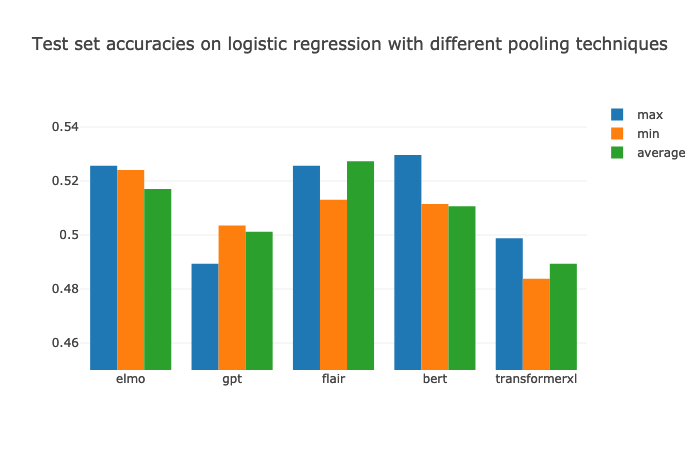
\includegraphics[scale=0.5]{poolingaccuracy}
    \caption{Comparing different pooling strategies.}
\end{figure}

\subsection{RQ2}
To answer the question which sequence length is optimal for neural classification, data with variable maximum lengths have been fed into bidirection LSTMs and convolutional neural networks.
For these maximum lengths, the lengths between two standard deviations from the median of the total word lengths per statement have been used, as is illustrated in figure 4. 
In this figure, the lowest maximum length, the median and the highest length are shown.

\begin{figure}
    \centering
    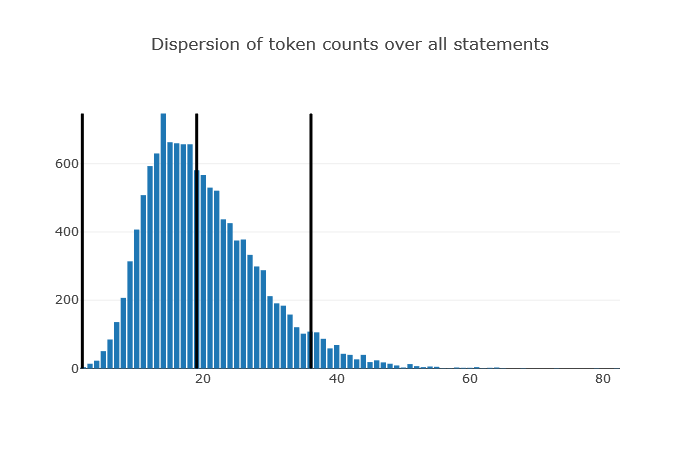
\includegraphics[scale=0.5]{wordlength}
    \caption{Total token counts per statement on the Liar dataset.}
\end{figure}

\begin{figure}[h]
    \centering
    \begin{subfigure}[b]{1\textwidth}
       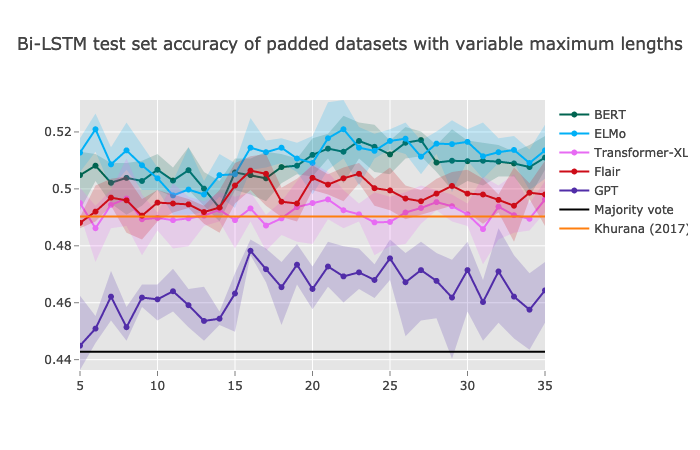
\includegraphics[width=1\linewidth]{bilstmaccuracies}
       \caption{Bidirectional LSTM accuracies.}
    \end{subfigure}
    
    \begin{subfigure}[b]{1\textwidth}
       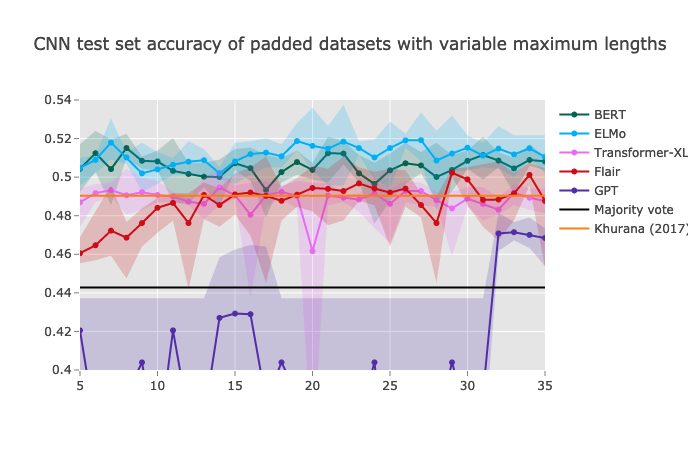
\includegraphics[width=1\linewidth]{cnnaccuracies}
       \caption{Convolutional neural network accuracies.}
    \end{subfigure}
    
    \caption{Test set accuracies with variable maximum lengths over neural network architectures.}
\end{figure}

In figure 5\todo{Check if this number is still correct}, the accuracies with different amounts of padding can be seen, compared to our 3 baselines.

\subsection{RQ3}
\textbf{How well do neural network classification architectures classify fake news compared to non-neural classification algorithms?}\\
The answer of this question will be given by comparing two linear classifiers with two neural classifiers. 

\begin{figure}[h]
    \centering
    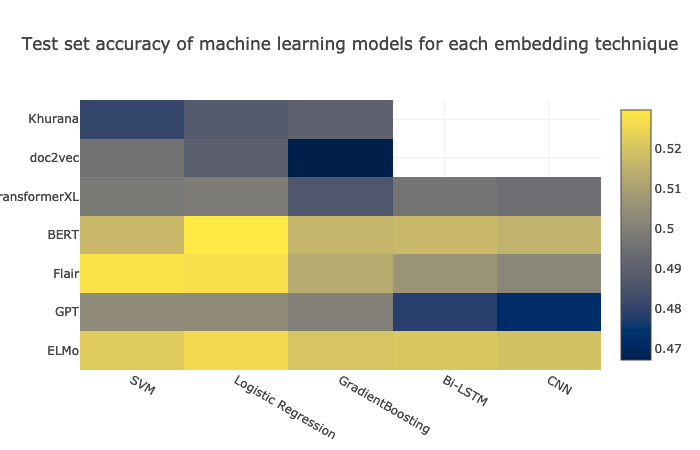
\includegraphics[scale=0.5]{linearvsneural}
    \caption{Comparing linear classifiers with neural classifiers.}
\end{figure}

\pagebreak
\section{Conclusions}
\label{sec:conc}

Hierin beantwoord je jouw hoofdvraag op basis van het eerder vergaarde bewijs.



\subsection{Acknowledgements}
Hier kan je bedanken wie je maar wilt.

% your refs

\pagebreak

\bibliographystyle{plain}
\bibliography{bibliography}

\appendix

%\input{appendix}
 
\end{document}
